%!TEX root = ../main/main.tex
\subsection{Análise do Fator}

A análise do componente principal apresentou quais variáveis são passíveis de melhor explicarem o que influencia no desempenho do curso no CPC. Foi apresentado o conjunto de variáveis e o perfil de cada componente. Contudo, é oportuno incluir mais uma camada de robustez à pesquisa pela aplicação da Análise do Fator -- AF ou (\textit{Factor Analysis} -- FA). \citeonline[p.~110--111]{larose2015data} destaca que, apesar de a ACP e AF serem técnicas de análise multivariada bem similares, a ACP deve ser em essência, um meio para a consecução da AF. 

De acordo com \citeonline[p.~93]{hair1998multivariate} a AF desempenha um papel importante na identificação das interações entre as variáveis por intermédio do agrupamento (em fatores) das mesmas de acordo com seu grau de relação. Esse procedimento permite a redução da dimensionalidade. Isso quer dizer que procura-se descrever um evento utilizando um conjunto menor de variáveis relativamente ao conjunto original estudado com o mínimo de perda de informação.

Vale ressaltar que as conclusões desta pesquisa tem perspectiva exploratória. Procura-se por meio do AF estabelecer uma estrutura nos dados do Enade utilizando este método como técnica de redução. Essa abordagem é diferente da confirmatória pois não são utilizados testes para se chegar a uma estrutura esperada com base em hipóteses. \Ibidem{hair1998multivariate}.

De acordo com \citeonline[p.~111]{larose2015data}, precedem a aplicação da AF os seguintes procedimentos: (i) padronização das variáveis; (ii) determinação dos vetores-Z (ou \textit{Z-vectors}) e (iii) a matriz de correlação.

Na figura \ref{fig: matriz-correlograma} vemos a reapresentação da matriz de correlação das variáveis preditoras agrupadas em \textit{clusters} de acordo com a intensidade de correlação. 

\begin{figure}[H]
		\centering
		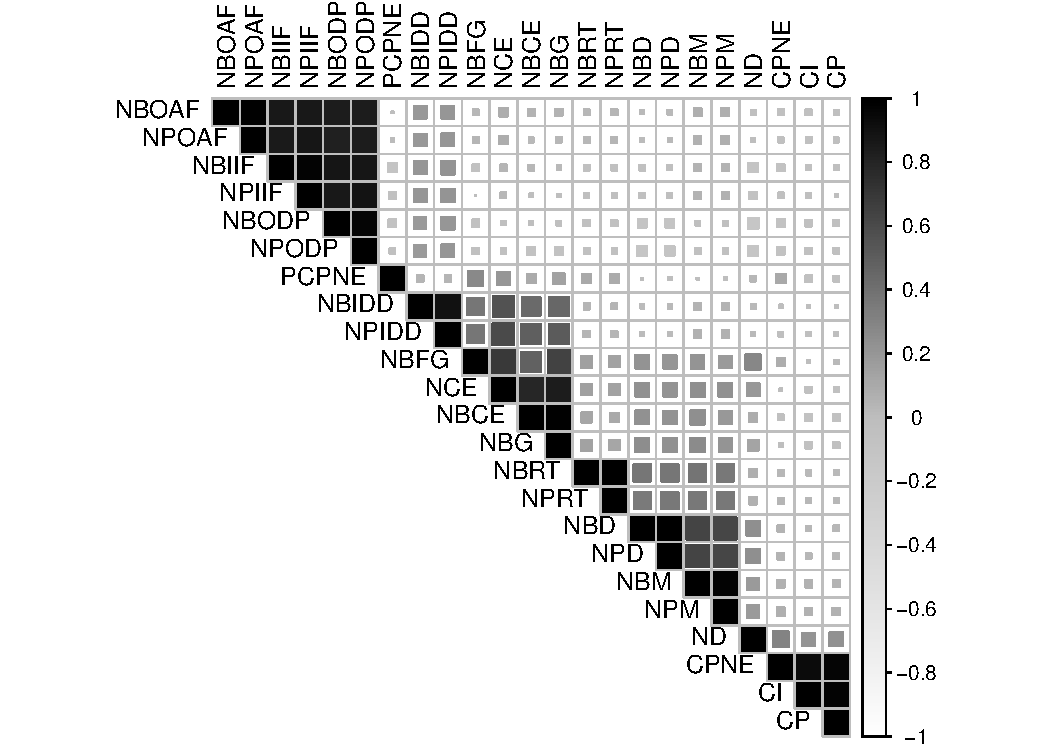
\includegraphics[scale=.75]{../../graficos/latex-graph-matriz-correlacao}
		\caption{Matriz correlograma}
		\label{fig: matriz-correlograma}
\end{figure}

Para que seja empregada de forma correta, a AF requer que as variáveis estejam minimamente correlacionadas. Neste sentido, \citeonline[p.~112]{larose2015data} recomendam a realização do teste de \textit{Esfericidade de Bartlett} para determinar se existe um nível mínimo de correlação como fase preliminar à aplicação da AF. Seguindo este autor, o referido teste foi realizado nos dados padronizados das variáveis do \textit{dataset} em questão. O resultado é apresentado na listagem \ref{lst:teste_de_bartlett}.
\pagebreak
\begin{lstlisting}[label={lst:teste_de_bartlett}, caption={Teste de Esfericidade de Bartlett}, captionpos=b]
$chisq
[1] 469552.9
$p.value
[1] 0
$df
[1] 300
\end{lstlisting}

O teste de Bartlett verifica a \textit{hipótese nula} de que a matriz de correlação é uma matriz identidade, sendo as variáveis portanto não correlacionadas. A principal informação deste teste é o valor de p (ou \textit{p-value}). Valores muito acima de 0.10 indicam que a aplicação do AF pode não ser adequada. Por outro, lado valores pequenos indicam que há evidências contra a hipótese nula, consequentemente validando o método. Como observado na saída acima, o \textit{p-value} é 0 o que indica que o AF pode ser aplicada.

Na listagem \ref{lst:loadings_fa_antes_rotacao} são apresentados os dois resultados da aplicação da função \lstinline{fa} sobre os dados padronizados. O primeiro resultado contém os \textit{eigenvalues} de cada variável preditora computada. O segundo contém os carregamentos (ou \textit{loadings}) juntamente à proporção de variância e variância acumulada.

\begin{lstlisting}[label={lst:loadings_fa_antes_rotacao}, captionpos=b, 
caption={Carregamentos da AF: o primeiro fator demonstra similaridade com o primeiro componente da ACP o que confirma a solidez e consistência das constatações até aqui verificadas.}]
 [1]  6.82829446  5.06102146  3.02305954  2.57594785  0.89229036  0.73263127  0.44322564  0.32873650  0.12874448
[10]  0.09205939  0.02032373 -0.01542126 -0.02141875 -0.04602155 -0.05979722 -0.08471119 -0.09794112 -0.11387848
[19] -0.13637542 -0.23237097 -0.27069873 -0.29403878 -0.29933457 -0.31091515 -0.65475511

Loadings:
      PA1    PA2    PA3    PA4   
CI            0.129  0.844  0.451
CP            0.128  0.866  0.470
NBFG   0.453  0.382 -0.135  0.247
NBCE   0.552  0.415 -0.294  0.297
NBG    0.596  0.461 -0.299  0.332
NCE    0.652  0.446 -0.285  0.365
NBODP  0.551 -0.753              
NPODP  0.545 -0.772  0.100       
NBIIF  0.613 -0.713  0.110       
NPIIF  0.614 -0.715  0.135       
NBOAF  0.641 -0.650  0.122       
NPOAF  0.633 -0.654  0.129       
CPNE          0.172  0.835  0.469
PCPNE         0.123              
NBIDD  0.583  0.103 -0.241  0.406
NPIDD  0.628  0.108 -0.267  0.431
ND     0.125  0.258  0.222       
NBM    0.462  0.423  0.264 -0.463
NPM    0.452  0.407  0.278 -0.463
NBD    0.420  0.493  0.242 -0.495
NPD    0.422  0.486  0.250 -0.498
NBRT   0.307  0.322  0.167 -0.342
NPRT   0.300  0.312  0.170 -0.340
CPCC   0.958  0.248              
CPCF   0.862  0.219              

                 PA1   PA2   PA3   PA4
SS loadings    6.828 5.061 3.023 2.576
Proportion Var 0.273 0.202 0.121 0.103
Cumulative Var 0.273 0.476 0.596 0.700
\end{lstlisting}

Observa-se que os quatro primeiros fatores computam uma variância de 68,4\% -- ligeiramente menor quando comparado à variância acumulada da mesma quantidade de componentes principais na fase de aplicação da ACP que foi de 72,3\%. É verificado também que, assim como na ACP, o primeiro fator é o que possui a maior variância.

Quanto a seleção de fatores, o mesmo critério foi utilizado em relação à escolha dos componentes na ACP: \textit{Scree plot} \cite[p.~109]{hair1998multivariate}. O gráfico da figura \ref{fig: fa-scree-plot} demonstra que a partir do 5º fator há uma tendência à estabilização em relação à variância explicada pelos fatores individuais.

\begin{figure}[H]
		\centering
		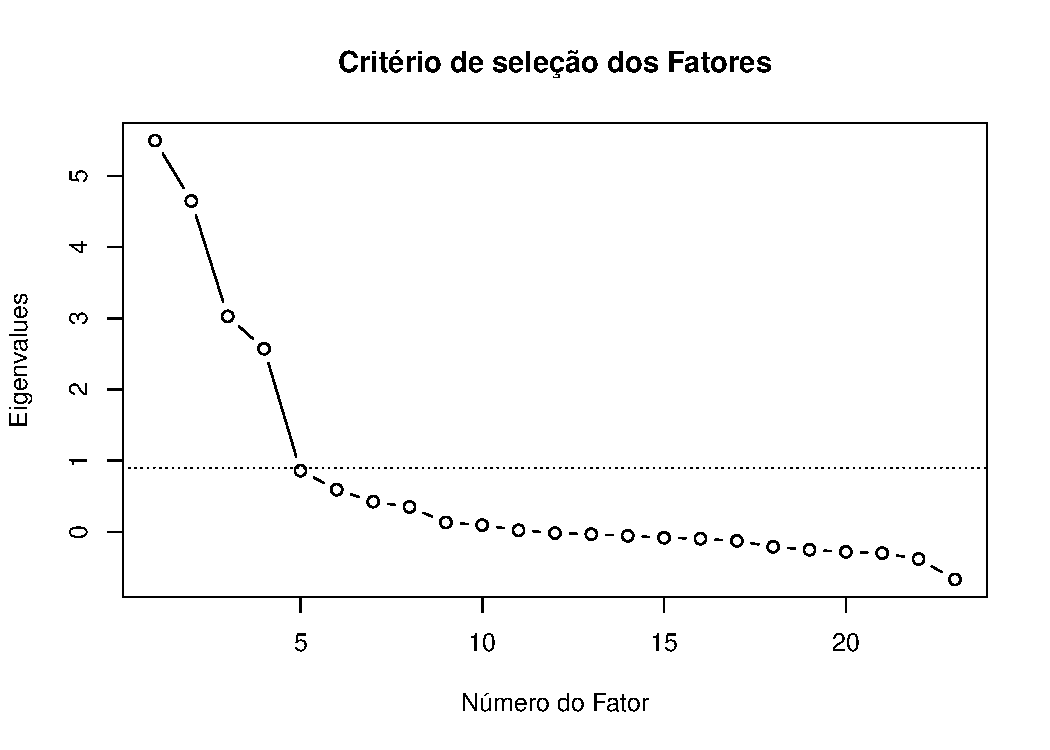
\includegraphics[scale=.75]{../../graficos/latex-graph-fa-scree-plot.pdf}
		\caption{Critério de seleção dos fatores: a partir do 5º fator, observa-se uma tendência de horizontalização da curva de variabilidade explicada pelos fatores, o que torna os fatores a partir desta contagem menos suscetíveis em participar de uma seleção.}
		\label{fig: fa-scree-plot}
\end{figure}

\subsubsection{Rotação dos Fatores}

A rotação dos fatores consiste em um elemento de validação da Análise do Fator. De acordo com \citeonline[p.~112]{hair1998multivariate}, a rotação serve para redistribuir as proporções de variância residuais dos fatores mais afastados para os iniciais. \citeonline[p.~114]{larose2015data} faz a analogia de um cientista tentando obter maior resolução em uma imagem ao ajustar o foco de seu microscópio.

\begin{lstlisting}[label={lst:loadings_fa_apos_rotacao}, caption={Carregamentos da AF após rotação}, captionpos=b]
Loadings:
      PA2    PA1    PA4    PA3   
CI                          0.965
CP                          0.993
NBFG          0.627  0.176       
NBCE          0.791  0.151       
NBG           0.857  0.168       
NCE           0.900  0.168       
NBODP  0.934                     
NPODP  0.947                     
NBIIF  0.947                     
NPIIF  0.953                     
NBOAF  0.919                     
NPOAF  0.918                     
CPNE                        0.972
PCPNE         0.169              
NBIDD  0.215  0.725              
NPIDD  0.233  0.779              
ND            0.133  0.212  0.255
NBM           0.122  0.811       
NPM           0.104  0.804       
NBD           0.114  0.841       
NPD           0.108  0.843       
NBRT                 0.580       
NPRT                 0.571       
CPCC   0.395  0.741  0.524       
CPCF   0.358  0.667  0.468       

                 PA2   PA1   PA4   PA3
SS loadings    5.672 4.814 4.056 2.946
Proportion Var 0.227 0.193 0.162 0.118
Cumulative Var 0.227 0.419 0.582 0.700

\end{lstlisting}

A rotação de fatores pode ser entendida como o esforço para obtenção da melhor configuração de variâncias no plano cartesiano. A listagem \ref{lst:loadings_fa_apos_rotacao} demonstra a rotação pelo método \textit{Varimax} que maximiza a variabilidade para cada coluna. Pela comparação com a listagem \ref{lst:loadings_fa_antes_rotacao}, percebe-se que variabilidades maiores são obtidas após a rotação.

%\subsubsection{Considerações sobre os Fatores}

%Enviado para a sessão Resultados, após comentário no Schoology em 10/7 às 9:39 am.
%É possível verificar grande semelhança nos resultados das análises multivariadas AF e ACP no que se refere à composição do conjunto de variáveis que representam a redução de dimensionalidade. Por esse motivo, entende-se o caráter corroborativo da AF em relação ao ACP nesta pesquisa. Em termos de perfis de variáveis para cada fator, os mesmos não diferem dos perfis elaborados para ACP.

\pagebreak